\section{Aufbau und Durchführung}
\subsection{Aufbau}
\label{sec:Aufbau}

Für diesen Versuch wird ein Ultraschallechoskop und eine $\SI{1}{\mega\hertz}$-Ultraschallsonde verwendet.
Das Echoskop befindet sich im Impuls-Echo-Modus.
Zudem kann die Sende- bzw. Empfangsfrequenz regelbar verstärkt werden.
Das Echoskop selbst ist an einen Rechner angeschlossen, über den verschiedene Scan-Modi ausgewählt und ausgewertet werden können.
Die Computersoftware ist in der Lage, A-Scans, B-Scans und TM-Scans darzustellen.\\
Beim A-Scan (Amplituden Scan) wird die Intensität in Volt in Abhängigkeit von der Eindringtiefe aufgetragen.\\
Der B-Scan (Brightness Scan) liefert ein zweidimensionales Bild, bei dem Helligkeitsstufen die Intensität widerspiegeln.\\
Mit dem TM-Scan (Time-Motion Scan) wird eine zeitliche Bildfolge mittels schneller Abtastung aufgenommen.\\
Die zu untersuchenden Objekte sind ein Acrylblock mit elf Durchbohrungen, dargestellt in Abbildung \ref{abb:1}, und ein Herzmodell bestehend aus einem zylindrischen Behälter, dessen Boden eine wölbbare Kreismembran ist.
\begin{figure}[H]
  \centering
  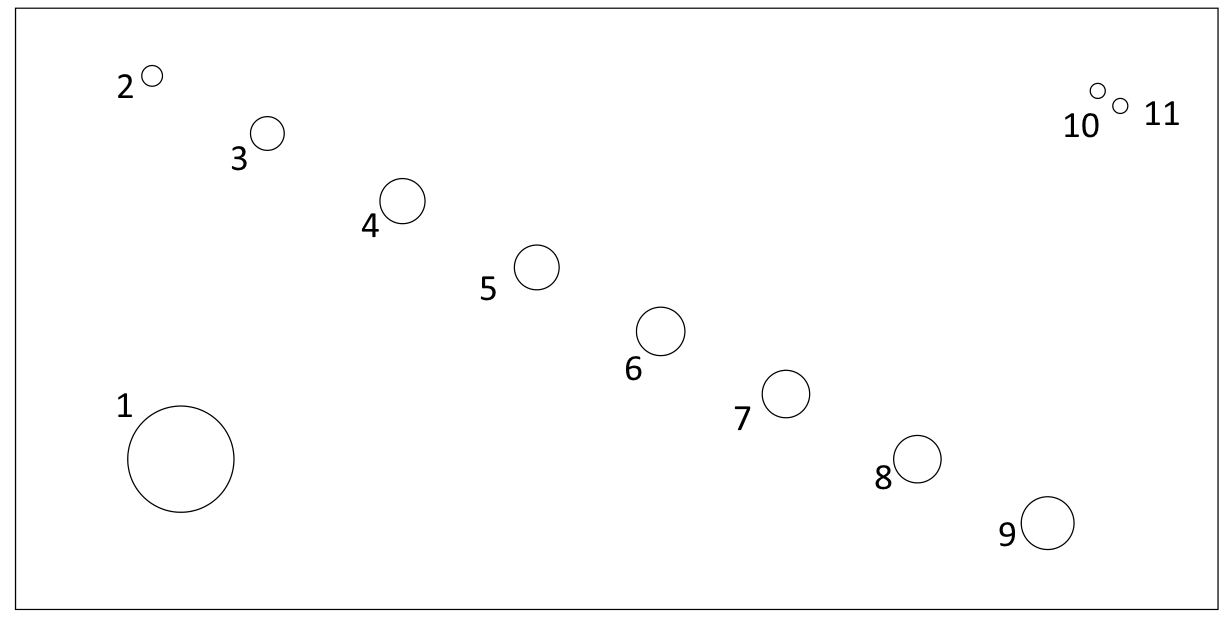
\includegraphics[height=6cm]{ressources/aufbau.png}
  \caption{Darstellung des Acrylblocks mit durchgängigen zylindrischen Ausbohrungen. \cite{skript}}
  \label{abb:1}
\end{figure}
